\chapter{Introduction}
\label{chp:introduction}
Development of complex, safety-critical systems requires an efficient way for engineers to ensure the correctness and reliability of the developed software. \acrlong{dsm} (\acrshort{dsm}) provides an approach to achieve this by enabling the creation of models that are closely aligned with the specific concepts and requirements of a particular domain. This approach usually includes automatic code generation, which significantly reduces the risk of faulty applications \cite{waldvogel_2022}.\\
By using \acrshort{dsm}, engineers can work more effectively, as it allows for the abstraction of complex system details into more manageable and understandable representations. This not only enhances productivity but also the overall quality and safety of the developed systems.\\
Models can be represented visually using block-diagrams to further simplify the development process. Furthermore, \acrshort{dsm} enables the reuse of domain-specific knowledge and components.\\
In safety-critical domains, such as avionics, the ability to visualize models and automatically generate code from them ensures that the software adheres to safety standards and reduces the likelihood of human errors during the development process.

However, \acrshort{dsm} can only be used without subsequent manual verification, if the \acrshort{dsm} tools work correctly. This can either be achieved through time intensive qualified software development processes, which ensure an accurate and reliable visualization of \acrshort{dsm} through the tool itself, or through the use of unverified \acrshort{dsm} tools followed by the subsequent use of a small visualization verification tool to ensure the correctness of the application.\\
In low-cost projects with high safety requirements, a cost-effective qualification method is crucial, highlighting the potential of the latter approach for a qualifiable graphical verification tool for use in \acrshort{dsm} \cite{waldvogel_annighoefer_models_2024}.

A typical use case for \acrshort{dsm} in avionics could be a door opening system. The system consists of a door, a motor, a sensor and a control unit. The door can be opened and closed by the motor, which is controlled by the control unit. The sensor detects whether the door is open or closed. The control unit receives the sensor data and controls the motor accordingly.\\
This system can be modeled using a block diagram, where the door, motor, sensors and control unit are represented as blocks, and the connections between them are represented as lines. Another diagram can be used to model the airplanes hardware components and their connections, such as the core processing units, remote data concentrators, sensors and actuators. A third diagram can be used to allocate the functions to the hardware components, as well as the connections between them.\\
This diagram-based approach allows users to visualize the system and its components, making it easier to understand and communicate. Diagram-based model editors include well established tools such as \textit{Simulink} and \textit{Enterprise Architect}, which are widely used in the industry.

\chapter{Fundamentals}
\label{chp:fundamentals}
The following chapter provides an overview of the fundamentals of the technologies and concepts used in this thesis. It covers the \acrlong{xgee} (\acrshort{xgee}), computer vision, \acrlong{dsm} (\acrshort{dsm}), the challenges in \acrshort{xgee}'s visualization verification and the state of the art in automatic diagram interpretation.

\section{\acrlong{xgee} (\acrshort{xgee})}
\label{sec:xgee}
\textit{\acrshort{xgee}} is a graphical model editor, which is currently under development at the Institute of Aircraft Systems. This editor is designed to facilitate the creation and modification of ecore-based models through a browser-based graphical user interface. Generally, \acrshort{xgee} can be used to work with any kind of model, but this thesis focuses on its use in aviation.\\
The primary objective of \acrshort{xgee} is to provide a user-friendly platform that allows engineers to efficiently design and visualize complex avionic systems, possibly working simultaneously on the same model. A demonstrator of \acrshort{xgee} is currently available online.\footnote{\url{https://xgee.de/en/}}\\
Within \acrshort{xgee}, three distinct types of \textit{tokens} are utilized across three specialized editors to represent various components of avionic models. These editors are:
\begin{itemize}
    \item signals
    \item vertices
    \item text labels
\end{itemize}
We consider \acrshort{xgee} editors for three layers of the \acrlong{oaam} (\acrshort{oaam}): the functions editor, the hardware editor and the allocations editor. \acrshort{oaam} supports additional layers such as the \textit{restrictions layer} and \textit{capabilities layer}, which are not considered in this thesis.\\
In \textit{\acrshort{xgee}}, each of the three editor models utilizes a unique set of \textit{.svg} files to represent different components within the avionic model. These editor models are the \textit{functions editor}, the \textit{hardware editor}, and the \textit{allocations editor}. An overview of these editors is provided in the following sections.

\subsection{Functions editor}
\label{sec:functions_editor}
\begin{figure}[h]
    \centering
    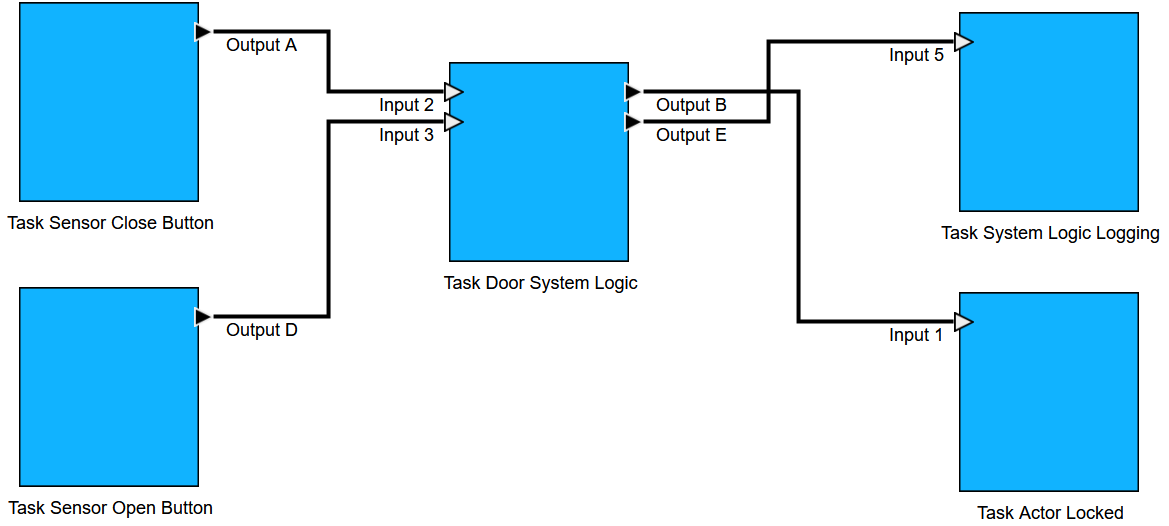
\includegraphics[width=0.4\textwidth]{pictures/functions_editor.png}
    \caption[Example of a diagram in the Functions editor]{Example of a diagram in the Functions editor.}
    \label{fig:functions_editor}
\end{figure}
The functions editor is used to define avionic functions and their interactions. Functions are represented as large blue boxes, with their interactions shown through black signals connecting inputs and outputs. Inputs and outputs are depicted as small black-and-white triangles located on the left and right edges of the function boxes. Inputs, outputs and functions have visible text labels (see \autoref{fig:functions_editor}).

\subsection{Hardware editor}
\label{sec:hardware_editor}
\begin{figure}[h]
    \centering
    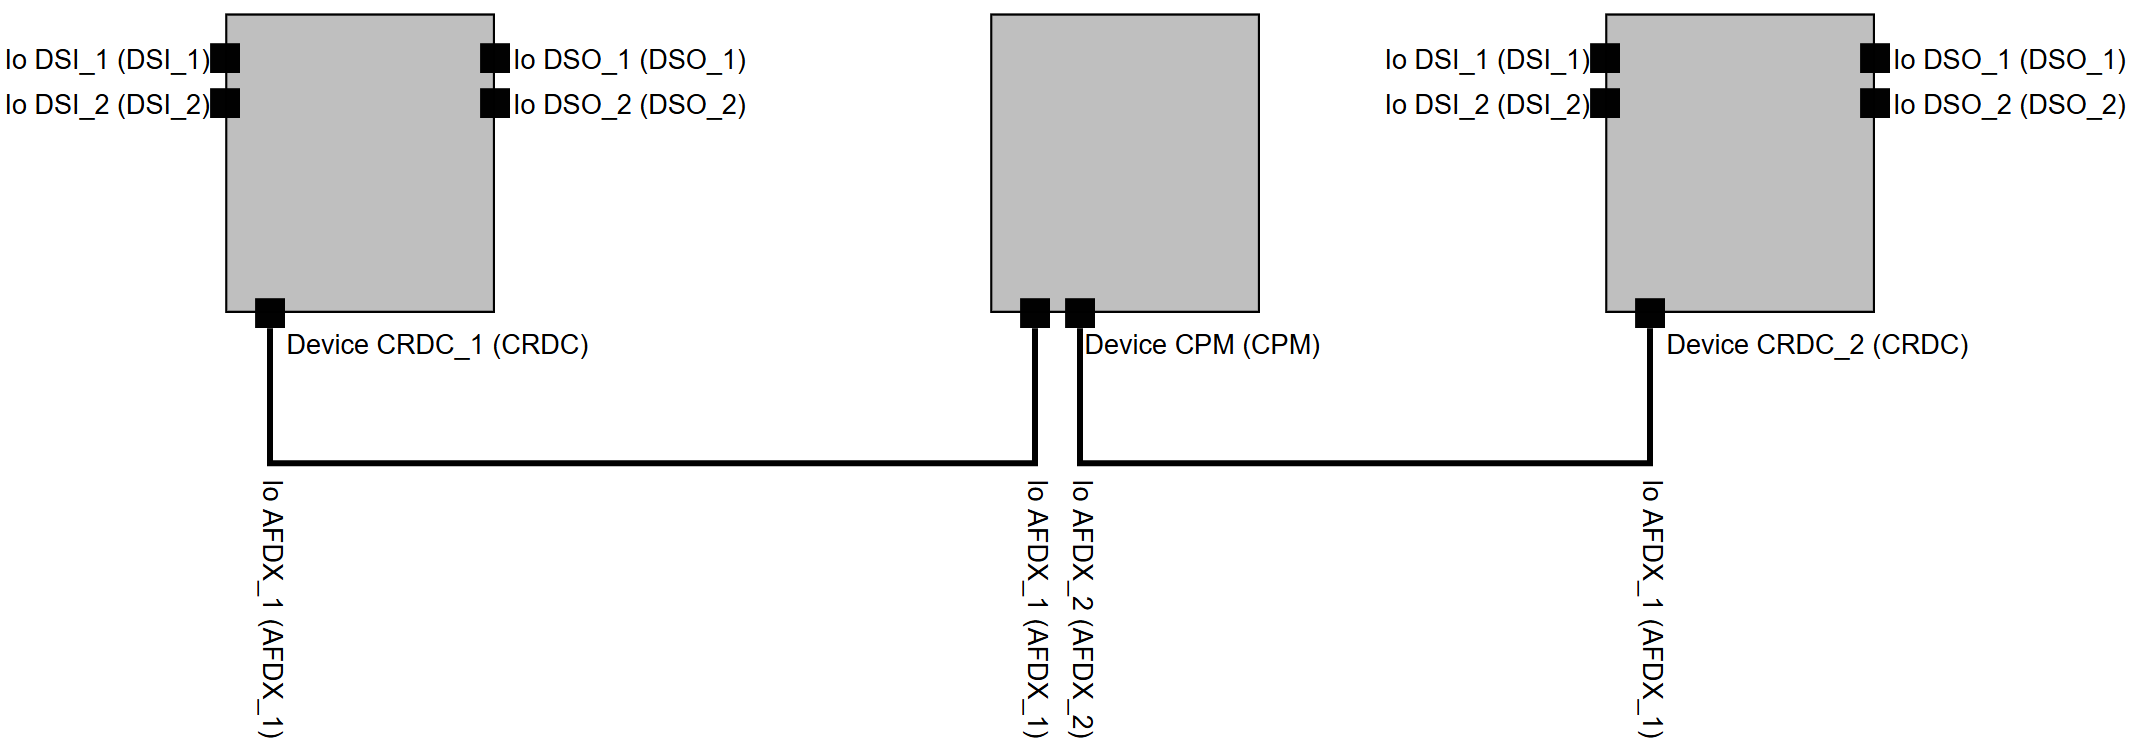
\includegraphics[width=0.4\textwidth]{pictures/hardware_editor.png}
    \caption[Example of a diagram in the Hardware editor]{Example of a diagram in the Hardware editor.}
    \label{fig:hardware_editor}
\end{figure}
The hardware editor is used to define hardware components and their physical connections. Hardware components are represented as large gray boxes, and their connections are illustrated as black signals linking \acrlong{io} (\acrshort{io}) ports. These \acrshort{io} ports appear as small black squares positioned along any edge of the hardware boxes. Like in the functions editor, \acrshort{io}s and devices have visible text labels (see \autoref{fig:hardware_editor}).

\subsection{Allocations editor}
\label{sec:allocations_editor}
\begin{figure}[h]
    \centering
    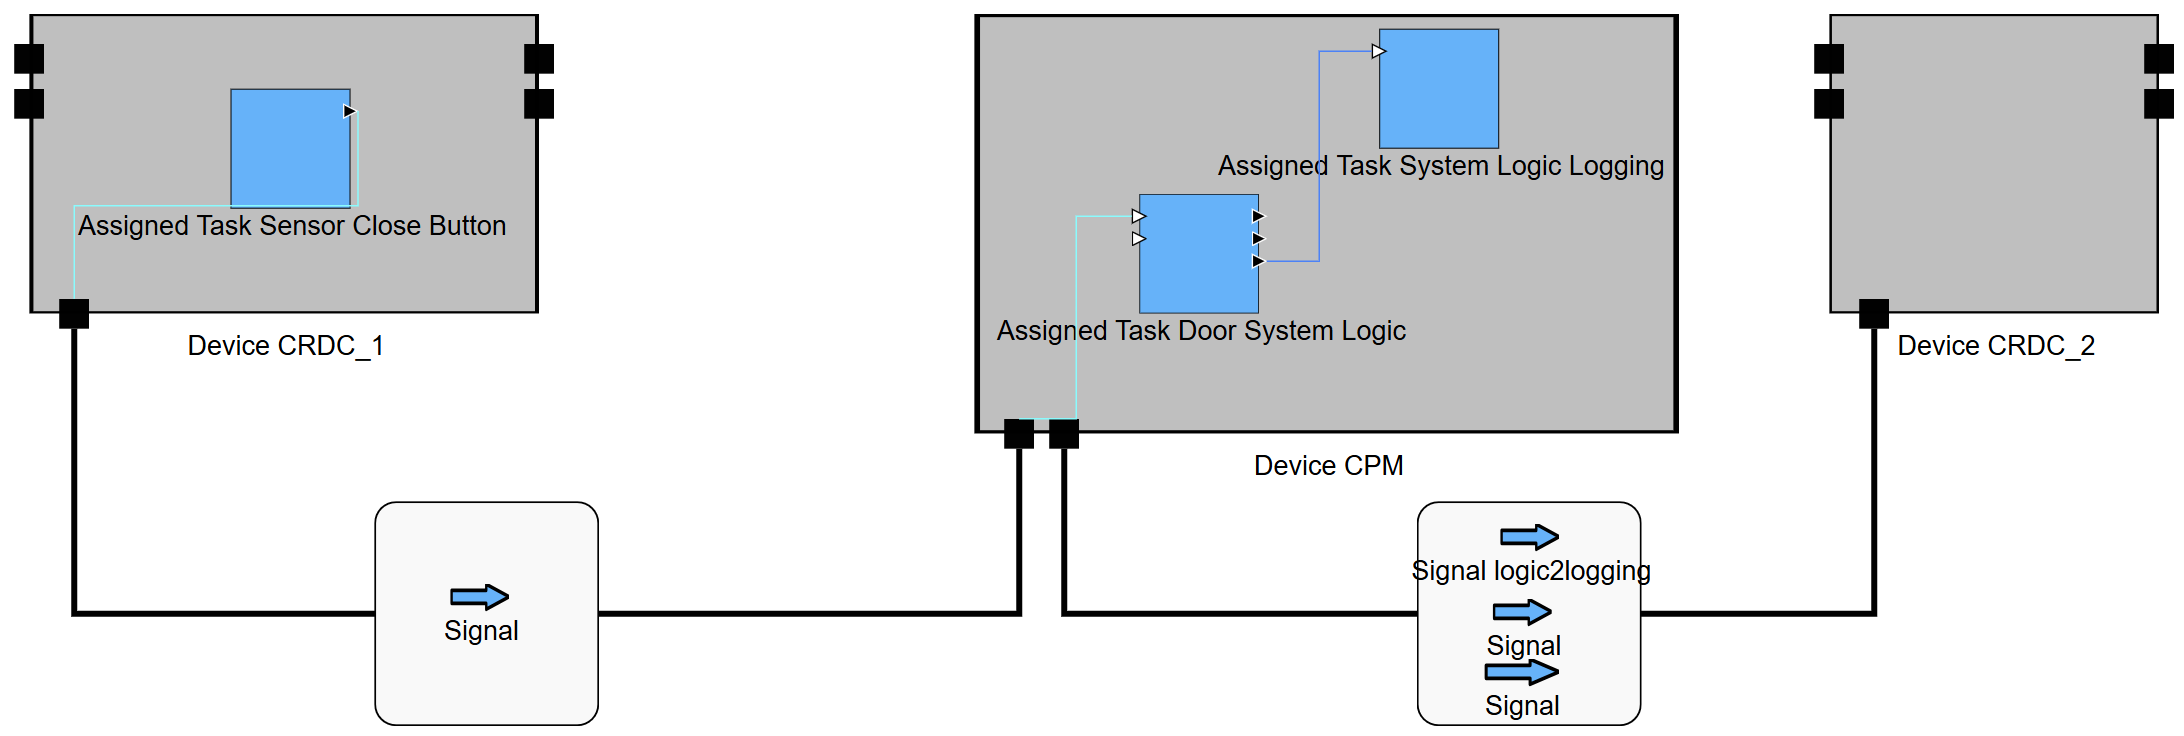
\includegraphics[width=0.4\textwidth]{pictures/allocations_editor.png}
    \caption[Example of a diagram in the Allocations editor]{Example of a diagram in the Allocations editor.}
    \label{fig:allocations_editor}
\end{figure}
The allocations editor is used to map functions to hardware components. Visually, it is simmilar to the hardware editor, with allocated functions represented as small blue boxes nested within larger gray hardware boxes. The specific signal transmissions between the hardware components are illustrated as white signal containers that overlap with the corresponding physical connections. These boxes contain the signals being transmitted through the corresponding connection. Inside the gray hardware boxes, connections between functions and \acrshort{io}'s, are illustrated as thin, color-coded signals. They represent the same connections proviously defined in the functions editor, but are now allocated to specific hardware components (see \autoref{fig:allocations_editor}).

This thesis builds upon the work of Andreas Waldvogel and Bj{\"o}rn Annigh{\"o}fer in \cite{waldvogel_annighoefer_models_2024} to further automate the verification process within \acrshort{xgee} by tokenizing a screenshot of the editor window. This means detecting the bounding boxes and token types of all elements of the diagram. To recognize and process the screenshot data, methods from the Python library \textit{\acrshort{opencv}} are being used.\\
The complete process of converting a screenshot of a block-diagram into meaningful error indications requires a series of individual steps, as shown in \autoref{fig:visualization_steps}.\\
By rebuilding a model from the recognized tokens and comparing it to the original, visualization errors become apparent and can be indicated to the user, including issues such as unclear signal intersections, signals being obscured by blocks, text labels being obscured by signals or blocks, blocks being scaled down to the point of disappearing, or blocks obscuring other blocks.\\
Fundamentally, this verification approach can be applied to any model-based application like Simulink. However, implementing the model comparison step would require much work, as the model has to be reconstructed from the recognized tokens, which is not trivial.\\
The goal of this thesis is to provide a tool that can be used to verify the correctness of the visualization of avionic models within \acrshort{xgee}'s functions and hardware editors, enabling engineers to work more effectively and with a higher degree of confidence.
\begin{figure}[h]
    \centering
    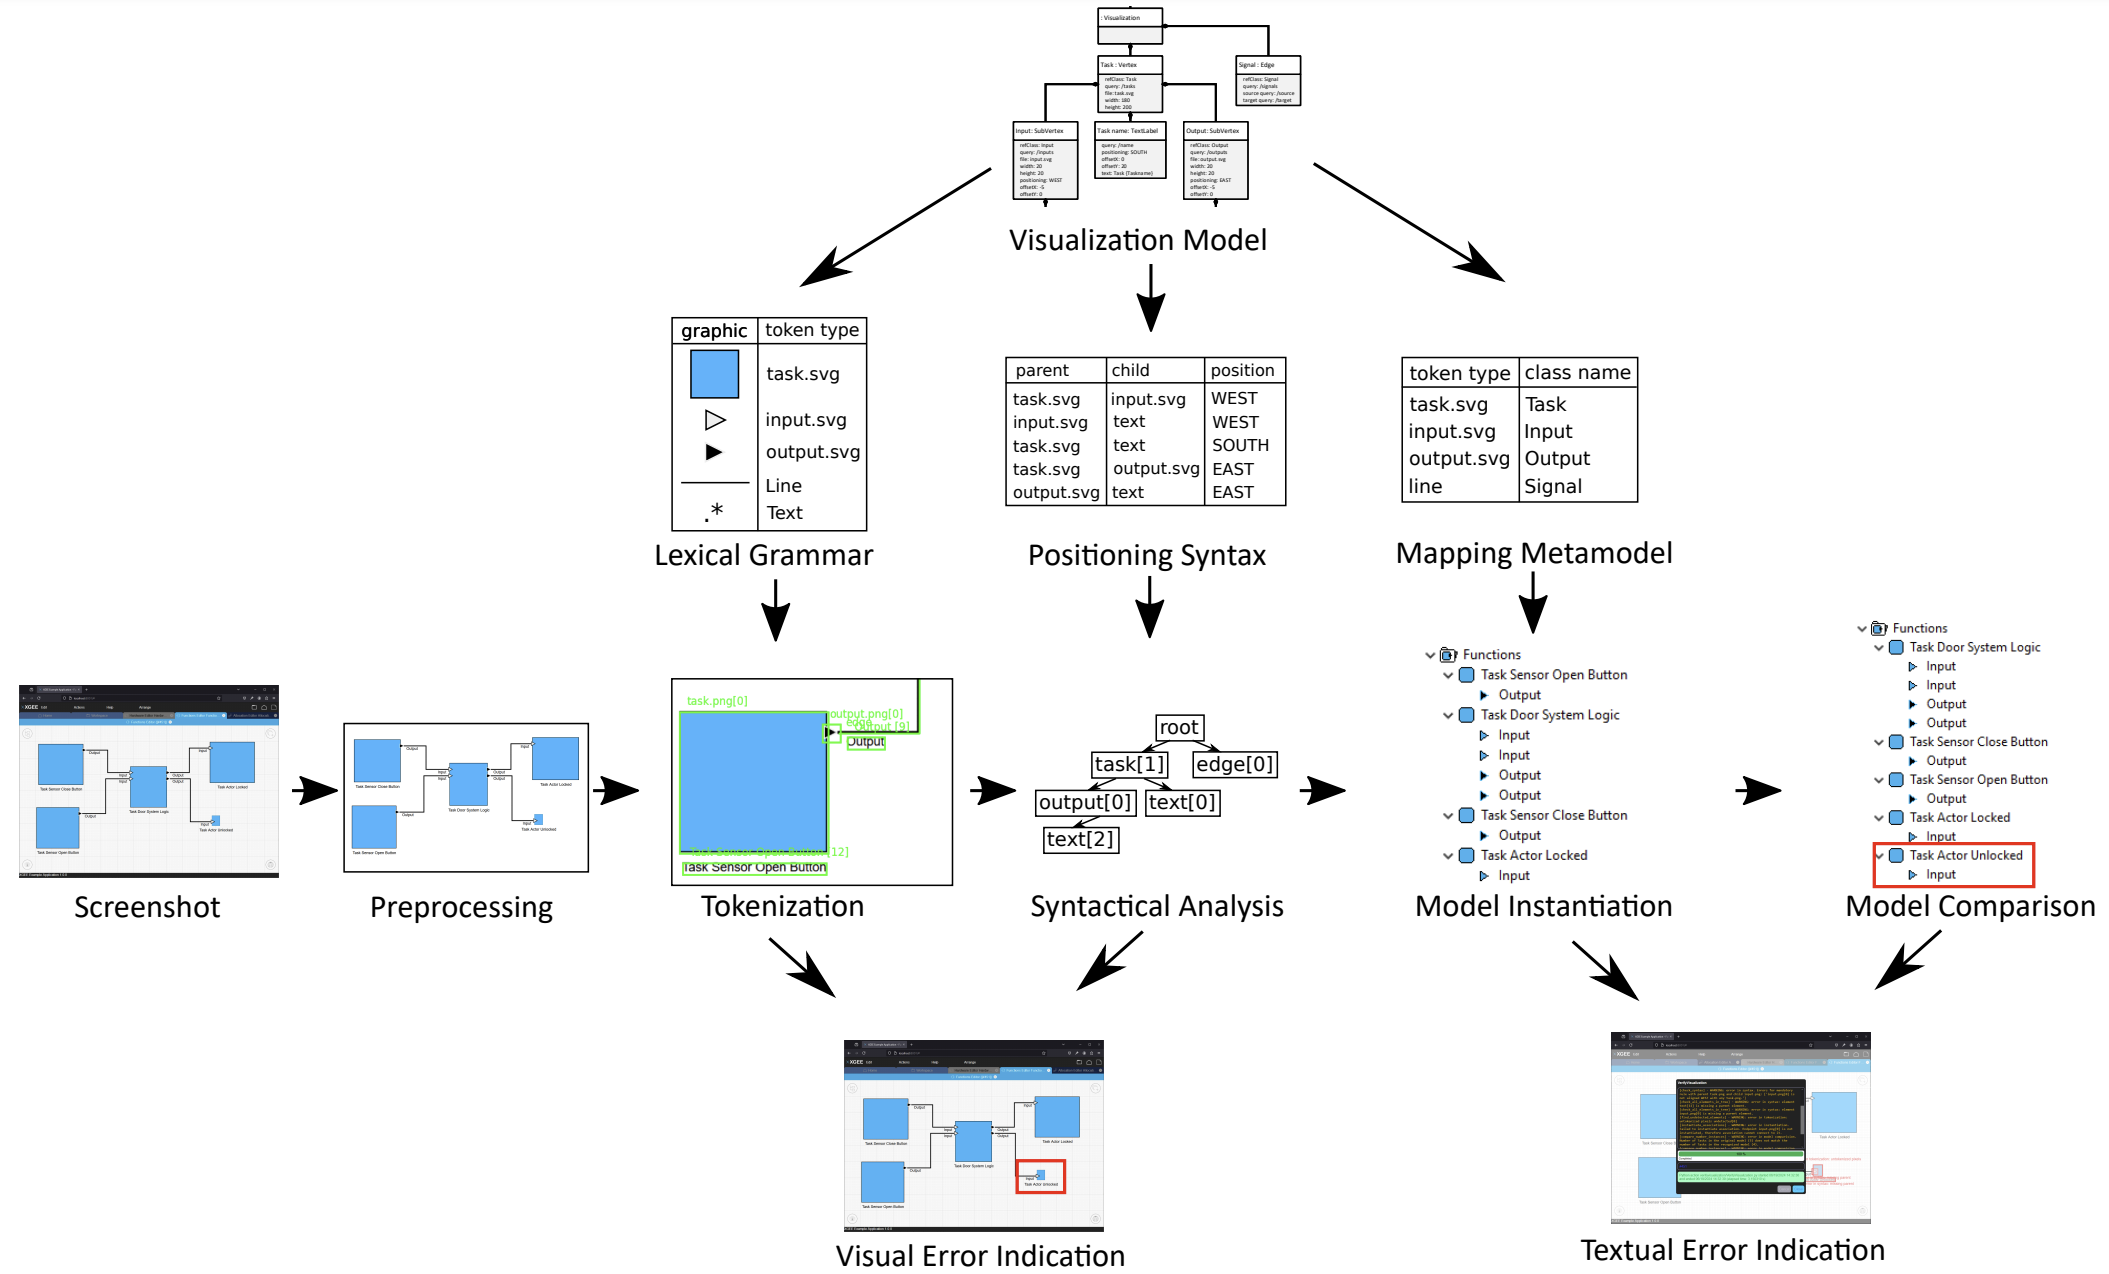
\includegraphics[width=0.9\textwidth]{pictures/visualization_steps.png}
    \caption[Steps in the visualization verification process]{Steps in the visualization verification process \cite{waldvogel_annighoefer_models_2024}.}
    \label{fig:visualization_steps}
\end{figure}

\section{Computer Vision}
\label{sec:computer_vision}
Humans have the remarkable ability to efficiently perceive and interpret visual information, extracting meaningful insights from their surroundings with ease. Tasks such as recognizing familiar faces, estimating distances, or identifying irregularities in a road surface may appear trivial to us, yet they present a significant challenge for computers to replicate.\\
Computer Vision is the field of mathematical models and approaches that enable computers to recover, interpret, and understand information from images or videos like humans. It encompasses a wide range of tasks, including image recognition, object detection, automation and more. It has numerous applications in a variety of fields, such as autonomous vehicles, facial recognition and medical imaging. Eventhough the field has made significant progress in recent years, many challenges such as handeling complex environments in real-time, detecting objects in low-light conditions or interpreting ambiguous data remain unsolved.\\
In avionic model development, visual representations of models are used to communicate complex systems and their interactions. To ensure correctness of these models, computer vision tools are used to interpret and verify the visual model representations, eliminating the need for manual verification.

\section{\acrlong{dsm}}
\label{sec:domain_specific_modeling}
When developing safety-critical real-world applications, such as an avionics system, \acrlong{oop} (\acrshort{oop}) enables developers to create complex systems by defining classes and objects that interact with each other. However, as the complexity of these systems increases, it becomes harder for many developers to collaborate on the same project, as they need to understand the entire system to make changes.\\
\begin{figure}[h]
    \centering
    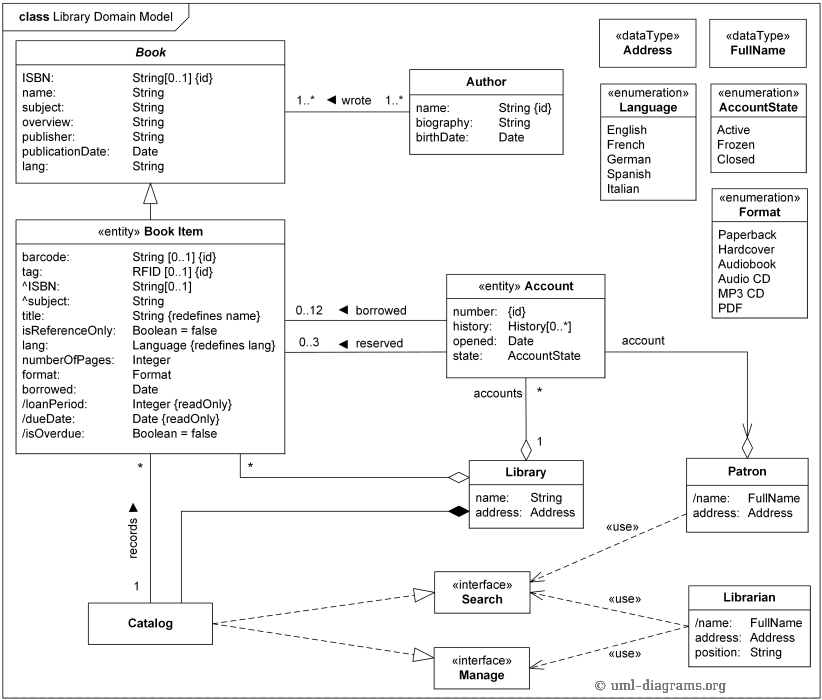
\includegraphics[width=0.6\textwidth]{pictures/uml_class_diagram.png}
    \caption[Example of an \acrshort{uml} class diagram]{Example of an \acrshort{uml} class diagram describing a library management system. In highly specialized domains, such as avionics, an \acrshort{uml} diagram might be too abstract to clearly represent the system. \cite{uml_diagrams_2016}}
    \label{fig:uml_diagram}
\end{figure}
The \acrlong{uml} (\acrshort{uml}) is a generic and source-code-independent \acrshort{oop} description language that can be used to model software systems. It provides a standardized way to visualize the design of a system using \acrshort{uml} diagrams, making it easier to understand and communicate. These diagrams consist of clearly defined elements specified in the \acrshort{uml} standard and can be directly converted to code through automatic code generation.\\
\autoref{fig:uml_diagram} shows an example \acrshort{uml} class diagram describing a library management system.\\
While \acrshort{uml} provides a standardized approach for modeling software systems in a general-purpose manner, it may not fully address the specific needs of highly specialized domains, such as avionics. Domain-Specific Modeling (\acrshort{dsm}) addresses this issue by enabling engineers to create models that are closely aligned with the concepts and requirements of a particular domain. For example, in avionics systems, \acrshort{dsm} might use specialized notation to represent specific aircraft components, such as sensors, actuators, or flight control systems, rather than relying on abstract classes and objects like \acrshort{uml}. This reduces the semantic gap between the model and the real-world implementation.\\
In most cases, a \acrlong{dsl} (\acrshort{dsl}) is developed by a small group of experts within a company or within a collaboration between companies and tailored to their unique needs, then used consistently throughout the organization to ensure uniformity and efficiency. This approach simplifies design processes and ensures that models are more easily validated, improving both reliability and safety, both critical requirements in the development of avionics systems.

\section{Challenges in \acrshort{xgee}'s visualization verification}
\label{sec:challenges_xgee_visualization_verification}
The \acrshort{xgee} editor is a browser-based model editor that, in our application, allows users to create and edit avionic models using a graphical interface but in general, \acrshort{xgee} can be used to edit anything that uses an ecore metamodel. For this thesis, we conside three editor models: the functions editor, the hardware editor and the allocations editor, each useing a different set of tokens to represent different elements of the model.\\
To verify the correctness of this visualization, a screenshot of the model is tokenized, meaning that the bounding boxes and token types of all elements of the diagram are detected. The recognized tokens are checked for correct syntax and unrecognized pixels. Then they are used to rebuild the model and compare it to the original, highlighting any visualization errors.\\
The primary challenge addressed in this paper is the accurate detection of these tokens. This includes handling intersecting and overlapping signals, obscured vertices and text labels, as well as large and complex models.\\
Furthermore, the integration of new methods for token detection into the existing codebase introduces an additional layer of complexity. 
Another challenge adressed in this thesis is to make the verification more versatile by enabeling it to change with the model. This is achieved by making the verification \textit{model-driven}, allowing the methods to query the current model for information and dynamically change their behavior based on it.

\section{State of the Art}
\label{sec:state_of_the_art}
Automatic diagram interpretation has been a topic of interest in the field of computer vision and \acrshort{dsm}. It could enable engineers to utilize diagrams that are currently only available as images or drawings, which would otherwise require manual reverse engineering. However, in large projects with consistent and well-maintained databases, most diagrams are already stored in usable formats, reducing the practical demand for automatic diagram interpretation in the industry. Consequently, no commercial tools for verified block diagram recognition are currently available on the market.

The work most similar to this thesis is presented in \cite{mani_haddad_constantini_douhard_li_poirier_2020}, which utilized a specifically trained \acrlong{cnn} to classify common symbols used in \textit{Piping and Instrumentation Diagrams}, achieving an accuracy of 90$\%$. They detected connecting lines using a graph search approach. By representing the pixels within the diagram image as a graph of black and white nodes, connecting lines can be identified by starting at any node corresponding to a symbol and traversing the diagram graph along its black nodes, keeping track of connected symbols along its path. For text detection, they used \textit{\acrshort{east}}, a text detectrion pipeline using a neural network. However, their method did not address the indication of uncertainties to the user. Instead, their primary goal was to digitize a database of diagrams to enable applications such as diagram search and machine learning-based predictive maintenance in the industry.\\
Recent research has focused on the recognition of handwritten diagrams, mathematical equations, flowcharts, and circuit diagrams. For example, \cite{wei_phung_bouzerdoum_bermak_2015} proposed a method for normalizing images captured by hand at arbitraty orientations to improve recognition accuracy and reliablity.\\
\cite{schaefer_keuper_stuckenschmidt_2021} used \textit{Arrow \acrshort{rcnn}}, a deep-learning model and an extension of the \textit{\acrlong{rcnn} (\acrshort{rcnn}) object detector} \cite{zhang2023dive} to detect and classify offline handwritten diagrams. \textit{\acrshort{rcnn}} is an object detection framework to identify bounding boxes around objects and classify each object into its respective category. On a scanned flowchart dataset, the model achieved an accuracy of 78.6$\%$, substantially improving the previous state of the art. However, their method was not designed recognize the diagrams structure or to adress the specific challenges of avionic model diagrams, particularly the need for validation and user feedback mechanisms.\\
Building on this work, \cite{fang_feng_cai_2022} proposed \textit{DrawnNet}, a \acrshort{cnn} and keypoint-based detector capable  of recognizing both symbols and diagram structures. Among other techniques, \textit{DrawnNet} leverages arrow direction predictions to enhance diagram interpretation.\\
\cite{yang_wang_zhang_li_wang_yang_shi_2024} proposed a framework for \acrlong{sld} (\acrshort{sld}) recognition, which are used in electrical engineering to represent power systems. Their methods include decomposing the diagram into seperate layers of electrical symbols and text labels to mitigate interference, using \acrshort{rcnn} to identify graphical symbols and the \textit{super-resolution} technique to improve text label recognition.

The approaches discussed above face challenges due to the inherent ambiguity of loosely defined graphical modeling languages and non-ideal photos of diagrams. A significant amount of effort is typically spent on recognizing various styles, but they often prioritize maximizing detection without considering the level of confidence in the results. In contrast, our approach takes a different direction. By leveraging the precise definition of a graphical \acrlong{dsl} (\acrshort{dsl}), we focus on a more structured verification process. Rather than attempting to recognize all elements, our goal is to highlight areas where uncertainty exists in the visualization, providing more meaningful and targeted feedback.
The methods proposed in this thesis are based on the work of \cite{waldvogel_annighoefer_models_2024}, which introduced a method for tokenizing and validating a screenshot of an avionic model within the \acrshort{xgee} editor. The aim of this thesis is to extend this work by improving the accuracy of token detection and integrating new methods for more complex detection tasks.